%%%%%%%%%%%%%%%%%%%%%%%%%%%%%%%%%%%%%%%%%%%%%%%%%%%%%%%%%%%%%%%%%%%%%%%%%%%%%%%%%%%%%%%%%%%%%
%									Chapitre 1												%
%%%%%%%%%%%%%%%%%%%%%%%%%%%%%%%%%%%%%%%%%%%%%%%%%%%%%%%%%%%%%%%%%%%%%%%%%%%%%%%%%%%%%%%%%%%%%
\chapter{Etat de l'art}
	\citationChap{
	We can only see a short distance ahead, but we can see plenty there that needs to be done.
	}{Alan Turing}
	\minitoc
	\newpage

%%%%%%%%%%%%%%%%%%%%%%%%%%%%%%%%%%%%%%%%%%%%%%%%%%%%%%%%%%%%%%%%%%%%%%%%%%%%%%%%%%%%%%%%%%%%%



% Début du chapitre

\section{La longue quête de l'Intelligence Artificielle}
\subsection{Une histoire d'échecs}
\subsection{L'inspiration biologique}
\subsection{L'émergence}

\section{La perception visuelle}
\subsection{Particularités de la vision}
\subsection{Cortex visuel humain}
\subsection{Méthodes classiques informatiques}

\newpage
\section{Réseaux neuronaux}
\subsection{Cartes auto organisatrices}

	Les cartes auto-organisatrices (aussi appellées réseaux de Kohonen) regroupent un ensemble de modèles qui a commencé par une publication de Teuvo Kohonen \cite{kohonen-som82}. Ces modèles sont caractérisés par leur capacité à projeter des données de façon ordonnée sur un espace d'une dimension plus faible (typiquement une ou deux dimensions). Cette réduction dimensionnelle donne ainsi une "carte" représentative des données qu'on lui a fourni, car les propriétés de voisinages sont conservées. Une des premières utilisation de ces cartes fut la représentation des phonèmes du finnois comme présenté dans la figure \ref{fig:img:phonemes}.

	\begin{figureth}
		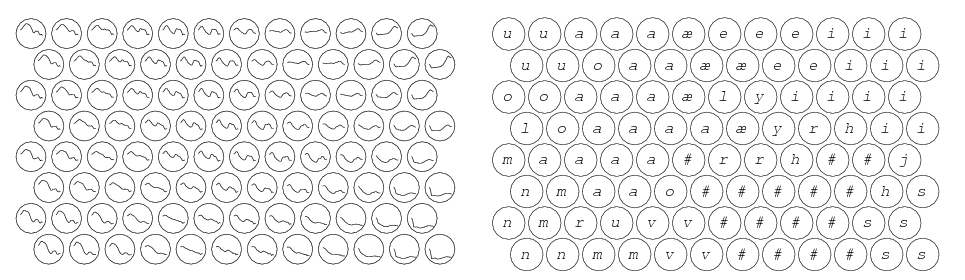
\includegraphics[width=\linewidth]{kohonen_phonemes}
		\caption[Phonème SOM]{Représentation des phonèmes du finnois par la première SOM. A gauche sont représentés les signaux sonores en haute dimension, et à droite leurs phonèmes correspondants. La réduction dimensionnelle provient de l'agencement de ces phonèmes sur la carte. Si ils sont proches entre eux dans leur espace d'entrée (signal), ils seront également proches dans la carte (la position des bulles). \textit{source : scholarpedia}}\label{fig:img:phonemes}

	\end{figureth}

	Le but premier de Kohonen était de présenter un modèle capable de représenter informatiquement l'organisation spatiale des informations dans le cortex humain \cite{kohonen-memory}. 
	
	Il s'inspira pour cela du concept neuroscientifique de colonnes corticales. Les colonnes corticales sont un groupe de neurones arrangées verticalement et qui réagissent tous au même stimulus.

\subsubsection{Evolutions et utilisation contemporaine}
	Il y a eu de nombreuses évolutions pendant les presque 40 années d'existence des SOM. En 2002, une bibliographie recensait 5384 articles scientifiques utilisant les SOM \cite{oja2003bibliography}. Ils étaient estimés à plus de 10000 en 2011 \cite{bilbiography-finuni}. Les domaines d'applications sont très variés, allant de l'image et la vidéo, par la parole et le traitement du signal, la médicine et la biologie, l'économie et la finance, de l'urbanisme et d'autres encore. Pour chacun de ces domaines il y a plusieurs types d'utilisations différentes de la SOM. Elle peut par exemple être utilisée en tant que méthode de visualisation capable de rendre humainement interprétable des données à très grande dimension et en les projetant sur des dimensions plus petites. Mais aussi pour faire des traitements sur des données, par exemple pour faire de la classification non supervisée de caractères, de chiffres ou de phonèmes, ou de la détection d'anomalies entre autres. \cite{cottrell2018self} est une revue récente évoquant les aspects les plus importants des SOM et présentant quelques applications typiques. 

	Evolutions et dérivés.

\subsection{Principes de fonctionnement}
\subsubsection{Préparation des données}

	Nous présentons dans cette section le fonctionnement de l'algorithme de la SOM que nous avons utilisé. Notre version est tout à fait classique et correspond à ce qui est communément utilisé dans la littérature.\\

	Les données présentées à la SOM doivent être numériques et sous forme de vecteurs. La taille des vecteurs peut être aussi grande que nécessaire, mais toutes les données de la bases doivent avoir la même taille de vecteur. Nous n'avons utilisé que des données normalisées, c'est à dire, dont la valeur est comprise entre 0 et 1 inclus. Par exemple pour apprendre des couleurs avec une SOM, on pourra représenter chaque couleur par un vecteur de taille 3, un élément par composante R,G et B par exemple et renormalisée pour être comprise entre 0 et 1. L'ordre de présentation des vecteur est aléatoire.

\subsubsection{Paramètres}

	La forme de la SOM dépend de plusieurs paramètres. Le premier est la dimensionalité. Les SOM peuvent aller d'une dimension de un à un nombre arbitrairement grand. Cependant, en pratique elles ne dépassent que rarement deux dimensions. La raison est que la visualisation est plus aisée en deux dimensions pour toutes les applications où cela en est le but premier. C'est aussi la taille idéale pour profiter de la réduction dimensionnelle sans pour autant augmenter de façon exponentielle les coûts en calculs à taille de carte égale. Une carte de 10 neurones de côté aura 100 neurones en deux dimensions et 1000 en 3 dimensions, les coûts en calculs étant proportionnels au nombre de neurones. Nous avons ainsi utilisé exclusivement des cartes bidimensionnelles dans nos expériences. Dans notre cas, nous avons également pris en compte la contrainte matérielle qui rend les toutes les dimensions supérieures à deux difficiles à implémenter efficacement dû à des coûts en communication accrus, car les circuits imprimés sont naturellement en deux dimensions.
	
	Un second choix important est ce que nous appellons la topologie de la SOM. Par topologie, nous entendons la forme des connections entre les neurones qui composent la SOM. Les deux topologies les plus communes pour les SOM sont en grille et hexagonale. Dans la topologie en grille chaque neurone a quatre voisins, un à chaque direction cardinale. En hexagone, chaque neurone a 6 voisins, formant un pavage hexagonal avec les neurones au centre des hexagones. Ces topologies sont deux dimensionnelles, mais il est possible de les rendre toriques ou sphériques. Nous n'explorererons pas cette possibilité dans cette thèse, car cela apporte en général plus de contraintes topologiques, c'est plus difficile pour une sphère de bien couvrir les données que pour une surface plane avec des degrés de libertés au extrémités. D'autres topologies plus exotiques existent et possèdent des propriétés intéressantes \cite{bernard2018np}, cependant nous avons dû nous limiter aux topologies classiques, les différences entre les topologies des SOM n'étant pas notre objet d'étude ici.

	Le dernier type de paramètre pour la SOM sont les paramètres numériques. Il y a parmi ceux-ci : La taille de la SOM, communément notée $n$. Elle défini le nombre de neurones par côté de la SOM. Le nombre total de neurones $N$ est obtenu à partir du carré des côtés : $n^2$. Dans le cas d'une SOM non-carrée, on notera $l$ et $h$ respectivement sa largeur et sa hauteur. Il y a aussi le coefficient d'apprentissage $\epsilon$ (epsilon), défini dans $]0,1[$. Il est décroissant linéairement tout au long de l'apprentissage, On notera dans cette thèse la valeur de départ et la valeur finale, toutes les valeurs intermédiaires seront extrapolées par la droite qui coupe ces deux points en fonction de l'étape courante de l'apprentissage. Le dernier paramètre est le coefficient de voisinage $\sigma$ (sigma), défini dans $[0,1[$. Il sert à définir l'impact des neurones voisins sur les poids du neurone courant. Plus il est élevé, plus les voisins ont un impact et plus la contrainte topologique sera forte. Inversement, une valeur de 0 pour ce paramètre enlève toute contrainte topologique et fait que la SOM se comportera comme un k-means. Comme pour le coefficient d'apprentissage, il décroit linéairement pendant l'apprentissage et nous n'indiquerons que les valeurs de départ et de fin.

\subsubsection{Apprentissage}

	

\subsubsection{Reconstruction}
	

	\subsection{GNG}
	GNGs

	Modern GNGs

	\subsection{DNF}

	Amari 1980

\newpage
\section{Matériel Neuromorphique}
\subsection{Processeurs}
\subsection{Caméra évènementielles}

\bibliographystyle{francaissc}
\bibliography{Chapitre1/Biblio}